\documentclass[12pt,a4paper]{article}
\usepackage[utf8]{inputenc}
\usepackage[russian]{babel}
\usepackage{amsmath}
\usepackage{amsfonts}
\usepackage{amssymb}
\usepackage{graphics}
\usepackage[pdftex]{graphicx}
\usepackage{lscape}
\author{Анастасия Тарасова}
\title{Отчет по лабораторной работе №1 :\\ \LaTeX{}, Git, GPG}
\begin{document}
\maketitle
\section{Система верстки \TeX{} и расширения \LaTeX{}}
\subsection{Цель работы}
Освоить систему верстки \TeX{} и сделать отчет.
\subsection{Ход работы}
В ходе работы был создан файл с расширением .tex, в котором содержатся команды текстовой разметки.
\subsubsection{Компиляция в командной строке}
Исходными данными для \LaTeX{} является обычный текстовый файл с расширением .tex. Его можно создать в любом текстовом редакторе (блокнот, Microsoft Word, встроенный редактор Far и пр.). Он содержит текст документа вместе с командами, указывающими \LaTeX{}, каким образом верстать текст.
Создание pdf-документа по входному файлу выполняется следующим образом:

\begin{itemize}
\item В командной строке необходимо выполнить команду

\verb+latex <имя входного файла без расширения>+

Команда преобразует входной файл в в файл формата dvi (Device Independent), пригодный к распечатке.
В настоящее время файлы формата dvi используются для предпросмотра итогового документа.
Файл dvi можно просмотреть при помощи утилиты Yap, распространяемой вместе с дистрибутивом MikTeX.
\item xdvi одна из программ DVI-драйверов, позволяющих отображать данные в формате
DVI в X Window системах

\verb+xdvi report1.dvi+

Результат показан на рисунке 1.
\begin{figure}[h!]
\centering
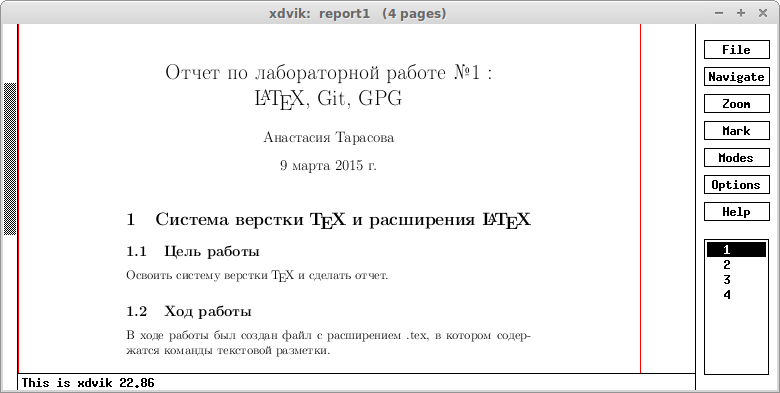
\includegraphics[scale=0.5]{res/xdvi}
\caption{Заппуск xdvi}
\end{figure}

\item
\verb+pdflatex report1.tex+

Команда создает итоговый pdf-документ.
\end{itemize}

\subsubsection{Оболочка TexMaker}
TexMaker - текстовый редактор, работающий с языком разметки LaTeX. TexMaker позволяет работать с фишками профессионального оформления. Внешний вид редактора представлен на рисунке 1. В редакторе TexMaker имеется возможность быстрой сборки и быстрого старта. Чтобы задать преамбулу документа, можно использовать помошника "Быстрый старт" (Меню "Помошник").Этот диалог позволяет задать главные особенности Вашего документа (класс, размер бумаги, кодировку...).
\begin{figure}[h!]
\centering
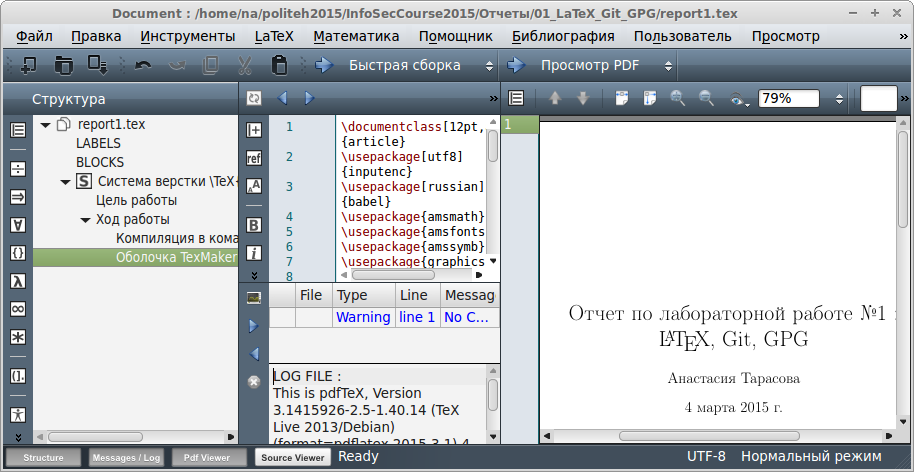
\includegraphics[scale=0.5]{res/texmaker}
\caption{Редактор TexMaker}
\end{figure}
\subsubsection{Классы документов}
В самом начале файла указывается класс документа, который задается командой\\\\
\verb+\documentclass[опции]{класс}+
\\\\Здесь класс определяет тип создаваемого документа. Опции изменяют поведение класса.\\\\
\verb+\documentclass[12pt,a4paper]{article}+ 
\\\\Эта строчка заставляет \LaTeX{} применить следующие правила для документа:

\begin{itemize}
\item[] Набирать документ как статью
\item[] Базовый размер шрифта - 12
\item[] Форматирование для печати на бумаге формата А4
\end{itemize}

\subsubsection{Подключаемые пакеты}
В процессе написание документа в некоторых областях базовый \LaTeX{} не сможет решить некоторые проблемы. В подключаемых пакетах можно указать особые настройки.
\\\\
\verb+\usepackage{lscape}+
\\\\
Данный пакет меняет положение страницы на ландшафтное

\subsubsection{Верстка формул}
\subsection{Выводы}
\LaTeX{} – это система набора текста, основанная на специальном скриптовом языке программирования. \LaTeX{} уже давно является стандартом де-факто при наборе научных статей, курсовых и дипломных работ, технических спецификаций, учебников и т. д. Главным преимуществом \LaTeX{} является абсолютно одинаковый внешний вид готовых страниц во всех операционных системах и непревзойденное до сих пор качество полиграфических текстов и математических формул. Кроме этого, скриптовый язык латеха – это универсальный язык для обмена формулами.

\newpage
\section{Система контроля версий Git}
\end{document}
